%%% Econ712: Macroeconomics I
%%% Fall 2020
%%% Danny Edgel
%%%
% Due on Canvas Thursday October 15, 11:59pm Central Time
%%%

%%%
%							PREAMBLE
%%%

\documentclass{article}

%%% declare packages
\usepackage{amsmath}
\usepackage{amssymb}
\usepackage{array}
\usepackage{bm}
\usepackage{changepage}
\usepackage{centernot}
\usepackage{graphicx}
\usepackage{fancyhdr}
	\fancyhf{} % sets both header and footer to nothing
	\renewcommand{\headrulewidth}{0pt}
    \rfoot{Edgel, \thepage}
    \pagestyle{fancy}
	
%%% define shortcuts for set notation
\newcommand{\N}{\mathbb{N}}
\newcommand{\Z}{\mathbb{Z}}
\newcommand{\R}{\mathbb{R}}
\newcommand{\Q}{\mathbb{Q}}
\newcommand{\lmt}{\underset{x\rightarrow\infty}{\text{lim }}}
\newcommand{\neglmt}{\underset{x\rightarrow-\infty}{\text{lim }}}
\newcommand{\zerolmt}{\underset{x\rightarrow 0}{\text{lim }}}
\newcommand{\loge}[1]{\text{ln}\left(#1\right)}
\newcommand{\usmax}[1]{\underset{\{#1\}}{\text{max }}}
\newcommand{\Mt}{M_{t+1}^t}
\renewcommand{\L}{\mathcal{L}}
\newcommand{\olq}{\overline{q}}

%%% define column vector command (from Michael Nattinger)
\newcount\colveccount
\newcommand*\colvec[1]{
        \global\colveccount#1
        \begin{pmatrix}
        \colvecnext
}
\def\colvecnext#1{
        #1
        \global\advance\colveccount-1
        \ifnum\colveccount>0
                \\
                \expandafter\colvecnext
        \else
                \end{pmatrix}
        \fi
}

%%% define function for drawing matrix augmentation lines
\newcommand\aug{\fboxsep=-\fboxrule\!\!\!\fbox{\strut}\!\!\!}

\makeatletter
\let\amsmath@bigm\bigm

\renewcommand{\bigm}[1]{%
  \ifcsname fenced@\string#1\endcsname
    \expandafter\@firstoftwo
  \else
    \expandafter\@secondoftwo
  \fi
  {\expandafter\amsmath@bigm\csname fenced@\string#1\endcsname}%
  {\amsmath@bigm#1}%
}


%________________________________________________________________%

\begin{document}

\title{	Problem Set \#6 }
\author{ 	Danny Edgel 					\\ 
			Econ 712: Macroeconomics I		\\
			Fall 2020						\\
		}
\maketitle\thispagestyle{empty}

%%%________________________________________________________________%%%

\noindent\textit{Collaborated with Sarah Bass, Emily Case, Michael Nattinger, and Alex Von Hafften}


%%%________________________________________________________________%%%

\section{(Non-) Commitment in a black-box example with discrete choice sets}
For clarity, the choice of the individual household is diplayed below. The household chooses between $\xi_k=x_L$ (left) and $\xi_k=x_H$ (right).
\begin{center}
	\begin{tabular}{|c|c|c|}
		\multicolumn{3}{c}{$\xi_k=x_L$}	\\ \hline
				& $x_L$ & $x_H$ \\ \hline 
		$y_L$	& 12 & 30 		\\ \hline
		$y_H$	& 0  & -1 		\\ \hline
	\end{tabular} \quad
	\begin{tabular}{|c|c|c|}
		\multicolumn{3}{c}{$\xi_k=x_H$}	\\ \hline
				& $x_L$ & $x_H$ \\ \hline 
		$y_L$	& -1 & 25 		\\ \hline
		$y_H$	& 30 & 24 		\\ \hline
	\end{tabular}
\end{center}

\begin{enumerate}
	\item The Ramsey outcome is reached when the government moves first and is thus able to optimize based on predicted household behavior. To find this outcome, we induct backward from the household problem, where households maximize utility at each $x_i$ and $y_j$:
		\[
			\xi_k = \underset{\xi\in X}{\text{argmax}}u(\xi,x,y) =
			\begin{cases}
				x_L, &	x_i = X_L\land y_j=y_L\\
				x_L, &	x_i = X_L\land y_j=y_H\\
				x_H, &	x_i = X_H\land y_j=y_H\\
				x_L, &	x_i = X_H\land y_j=y_L
			\end{cases}
		\]
		The government then chooses $y_j$ to maximize utility, given the HH solution and $\xi_k=x_i$. If the government chooses $y_L$, then households will chose $x_L$, resulting in a total utility of 12. If the government chooses $y_H$, then households will choose $x_H$, resulting in a total utilty of 24. Thus, $(x_H,x_H,y_H)$ is the Ramsey outcome.
		\medskip \\
		In the no-commitment outcome, households move first, choosing $\xi_k$ after inducting backward from the government's response to their choice. After households choose, government will be faced with maximizing total utility given $\xi_k=x_i$:
		\begin{center}
			\begin{tabular}{|c|c|c|}
				\multicolumn{3}{c}{$\xi_k=x_i$}	\\ \hline
						& $x_L$ & $x_H$ \\ \hline 
				$y_L$	& 12 & 25 		\\ \hline
				$y_H$	& 0  & 24 		\\ \hline
			\end{tabular} 
		\end{center}
		$y_L$ clearly dominates $y_H$, so households maximize utility assuming that $y_j=y_L$:
		\begin{center}
			\begin{tabular}{|c|c|c|}
					\multicolumn{3}{c}{$x_i$}	\\ \hline
							& $x_L$ & $x_H$ 	\\ \hline 
				$\xi_k=x_L$	& 12 	& 30 		\\ \hline
				$\xi_k=x_H$	& -1  	& 25 		\\ \hline
			\end{tabular} 
		\end{center}
		Regardless of $x_i$, households will be better-off choosing $x_L$, so the equilibrium in this case is $(x_L,x_L,y_L)$.
		
	\item In a repeated economy, the Ramsey outcome cannot be supported because the government can achieve a higher level of utility by deviating from $(x_H,x_H,y_H)$ to choose $y_L$ such that $u(x_H,x_H,y_L)=25$. It would choose to do so in the final period, knowing that there will not be an opportunity for households to respond by moving to $(x_L,x_L,y_L)$, where utility is lower, at 12. Households know that this is the government's optimal choice, so they factor this into their maximization problem by choosing $x_L$ in the fourth period. Governments then anticipate this in the third period, and so on. As a result, there is no period where the Ramsey equilibrium can be supported.
	
	\item  The tables below display the full incentive structure of the agents in this economy. The pure strategy Nash equilibria are $(x_{LL},x_{LL},y_{LL})$ and $(x_L,x_L,y_L)$, since at these bundles, neither households nor the government can inprove household utility unilaterally.
		\begin{center}
			\begin{tabular}{|c|c|c|c|}
				\multicolumn{4}{c}{$\xi_k=x_{LL}$}	\\ \hline
						&$x_{LL}$ & $x_L$ & $x_H$ \\ \hline 
			$y_{LL}$	& 2 	 & 30 	 & 30	\\ \hline
			$y_L$		& 1 	 & -1 	 & 30	\\ \hline
			$y_H$		& -1  	 & 30 	 & -1	\\ \hline
			\end{tabular} \quad
			\begin{tabular}{|c|c|c|c|}
				\multicolumn{4}{c}{$\xi_k=x_L$}	\\ \hline
						&$x_{LL}$ & $x_L$ & $x_H$ \\ \hline 
			$y_{LL}$	& -1 	 & 6 	 & 30	\\ \hline
			$y_L$		& 30 	 & 12 	 & 30	\\ \hline
			$y_H$		& 30  	 & 0 	 & -1	\\ \hline
			\end{tabular} \quad
			\begin{tabular}{|c|c|c|c|}
				\multicolumn{4}{c}{$\xi_k=x_H$}	\\ \hline
						&$x_{LL}$ & $x_L$ & $x_H$ \\ \hline 
			$y_{LL}$	& -1 	 & 30 	 & 10	\\ \hline
			$y_L$		& 30 	 & -1 	 & 25	\\ \hline
			$y_H$		& 30  	 & 30 	 & 24	\\ \hline
			\end{tabular}
		\end{center}
		Households and the government have the following problems:
		\begin{align*}
			&\usmax{\xi_k^1,\xi_k^2,\xi_k^3}u(\xi_k^1,x_i^1,y_j^1) + \beta u(\xi_k^2,x_i^2,y_j^2) + \beta^2u(\xi_k^3,x_i^3,y_j^3) 	&\text{(Household Problem)}	\\
			&\usmax{y_j^1,y_j^2,y_j^3}u(x_i^1,x_i^1,y_j^1) + \beta u(x_i^2,x_i^2,y_j^2) + \beta^2u(x_i^3,x_i^3,y_j^3) 				&\text{(Government Problem)}
		\end{align*}
		In this three-period economy with discounted utility where $\beta=0.9$, it is possible for the Ramsey equilibrium to be supported in the first and second periods if the households undertake a strategy to use the lower-utility equilibrium, $(x_{LL},x_{LL},y_{LL})$, as a punishing equilibrium for any premature deviation by the government from the Ramsey equilibrium. Consider a strategy where households expect the government to deviate from the Ramsey equilibirum in the final period but choose $x_{LL}$ if it does so before that. The household strategy is then $(x_H,x_H,x_L)$. 
		\medskip \\
		The govenment optimizes $u$ by choosing $y_j^t$ in each period knowing that choosing $y_L$ for any $t<3$ will result in households choosing $x_{LL}$ for all remaining periods. The government, then, chooses the utility-maximizing strategy from the following options:
		\begin{align*}
			(y_L,y_{LL},y_{LL}):\text{ }& u(x_H,x_H,y_L) + \beta u(x_{LL},x_{LL},y_{LL}) + \beta^2 u(y_{LL},x_{LL},x_{LL}) \\
										& = 25 + (0.9)2 + (0.81)2 	= 28.42	\\
			(y_H,y_L,y_{LL}):\text{ }	& u(x_H,x_H,y_H) + \beta u(x_H,x_H,y_H) + \beta^2 u(y_{LL},x_{LL},x_{LL}) 	 \\
										& = 24 + (0.9)25 + (0.81)2 	= 48.12 \\
			(y_H,y_H,y_L):\text{ }		& u(x_H,x_H,y_H) + \beta u(x_H,x_H,y_H) + \beta^2 u(x_H,x_H,y_H) 		 \\
										& = 24 + (0.9)25 + (0.81)12	= 56.22
		\end{align*}
		Thus, the government's optimal response to the household's optimal strategy is to remain on the equilibrium path and not prematurely deviate.
\end{enumerate}

%%%________________________________________________________________%%%
\pagebreak
\section{Static taxation}
For a unit measure of households with preferences over leisure ($l$), private consumption ($c$), and public goods ($g$), let utility be defined by
\[
	u(l,c,g) = \loge{l} + \loge{\alpha + c} + \loge{\alpha + g}\text{, }\alpha\in(0,0.5) 
\]
Assume each household is endowed with one unit of time, which can be split between labor, $\ell$, or leisure, $l$, where the government taxes labor proportionally to provide public goods, i.e. $g=\tau\ell$. One unit of labor, net of taxes, is worth one unit of consumption such that $(1-\tau)\ell = c$. Finally, the economy's resource contraint is:
\[
	\overline{l} + g + \overline{c} = 1
\]
Where $\overline{l}$ and $\overline{c}$ are aggregate leisure and consumption, respectively. In terms of labor, the resource constraint is:
\[
	\overline{\ell} - \overline{c} = g
\]
Where $\overline{\ell}$ is aggregate labor.

\begin{enumerate}
	\item Given that we have a unit measure of households, for the social planner, $\ell=\overline{\ell}$ and $c=\overline{c}$. The social planner's problem, then, is:
		\[
			\usmax{\ell,c,g}\loge{1-\ell} + \loge{\alpha + c} + \loge{\alpha + g}\text{, s.t. }\ell-c=g\text{, }\tau\ell=g
		\]
		Which, using the constraints, can be written as an unconstrained problem in terms of only $\tau$ and $\ell$:
		\[
			\usmax{\ell,\tau}\loge{1-\ell} + \loge{\alpha + (1-\tau)\ell} + \loge{\alpha + \tau\ell}	
		\]
		Where the first-order condition for $\tau$ yields
		\begin{align*}
			\frac{-\ell}{\alpha + (1-\tau)\ell} + \frac{\ell}{\alpha + \ell\tau} &= 0	\\
			\alpha + \ell\tau &= \alpha + (1-\tau)\ell \\
			2\ell\tau &= \ell \\
			\tau &= \frac{1}{2}
		\end{align*}
		Combining this optimal value for $\tau$ with the FOC for $\ell$ gives:
		\begin{align*}
			\frac{-1}{1-\ell} + \frac{1-\tau}{\alpha + (1-\tau)\ell}  + \frac{\tau}{\alpha + \ell\tau} &= 0	\\
			\frac{1}{2\alpha + \ell} + \frac{1}{2\alpha + \ell} &= \frac{1}{1-\ell}	\\
			\frac{2}{2\alpha + \ell} &= \frac{1}{1-\ell}	\\
			2\alpha + \ell &= 2 - 2\ell \\
			\ell &= \frac{2}{3}\left(1-\alpha\right)
		\end{align*}
		Thus, the social planner's allocation, which maximizes aggregate utility, is 
		\[
			{\{l,c,g,\tau\}=\left\{\frac{1}{3}\left(1-2\alpha\right),\frac{1}{3}\left(1-\alpha\right),\frac{1}{3}\left(1-\alpha\right),\frac{1}{2} \right\}}
		\]
		
	\item The Ramsey outcome occurs when the government has commitment/moves first. It is derived by inducting backward from the household's response to the government's choice of $\tau$, in which household's face the problem:
		\[
			\usmax{\ell,c}\loge{1-\ell} + \loge{\alpha + c} + \loge{\alpha + g}\text{, s.t. }c=(1-\tau)\ell
		\]
		Substituting the right side of the budget constraint for $c$ turns this into an unconstrained problem of a single choice variable, $\ell$. The FOC for $\ell$ is:
		\begin{align*}
			\frac{-1}{1-\ell} + \frac{1-\tau}{\alpha + (1-\tau)\ell}  &= 0	\\
			\frac{\alpha + (1-\tau)\ell}{1-\tau}&= 1-\ell  \\
			(1-\tau)(1-\ell) &= \alpha + (1-\tau)\ell \\
			1-\tau-2(1-\tau)\ell &= \alpha \\
			\ell &= \frac{1-\tau-\alpha}{2(1-\tau)}
		\end{align*}
		Which gives the optimal household choice of $c$, $\ell$, and $l$, based on the government's chosen $\tau$, as:
		\[
			\{c,\ell,l\} = \left\{\frac{1}{2}\left(1-\tau-\alpha\right),\frac{1-\tau-\alpha}{2(1-\tau)},\frac{1-\tau+\alpha}{2(1-\tau)} \right\}
		\]
		The government then factors the household's optimal choice into its choice of $\tau$. Substituting the household's choice of each variable into the utility function allows us to solve utility as a function of only $\tau$:
		\begin{align*}
			u(\tau) &= \loge{\frac{1-\tau+\alpha}{2(1-\tau)} } + \loge{\alpha + frac{1}{2}\left(1-\tau-\alpha\right)} + \loge{\alpha + \tau\frac{1-\tau-\alpha}{2(1-\tau)}} \\
					&= \loge{1-\tau+\alpha} - \loge{2} - \loge{1-\tau} + \loge{\frac{1}{2}(1-\tau+\alpha)} +
					   \loge{\frac{2\alpha + (1-3\alpha)\tau-\tau^2}{2(1-\tau)}} \\
					&= 2\loge{1-\tau+\alpha} + \loge{2\alpha + (1-3\alpha)\tau-\tau^2} - 2\loge{1-\tau} - 3\loge{2}
		\end{align*}
		Which has the first order condition:
		\begin{align*}
			\frac{\partial u}{\partial\tau} &= \frac{-2}{1-\tau+\alpha} + \frac{1-3\alpha - 2\tau}{2\alpha + (1-3\alpha)\tau-\tau^2} + \frac{2}{1-\tau} = 0
		\end{align*}
		This does not have an analytical solution (or at least not one that one can reasonably request in a problem set), but I solved for each value of $\alpha$ in the attached code. The Ramsey equilibrium allocation is displayed in the chart below.
		\begin{center}
			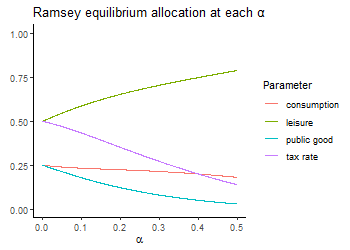
\includegraphics[scale=.8]{figure1.png}
		\end{center}
		
	\item In the no-commitment scenario, households move first after anticipating the government's behavior. Since the government seeks to maximize aggregate utility, the government would choose the social planner's allocation, $\tau=\frac{1}{2}$. Households would respond by maximizing their own utility, given this tax rate. Using the known optimal household values from 2 and plugging in $\tau=\frac{1}{2}$, we get:
	\[
		{\{l,c,g,\tau\}=\left\{\frac{1}{2}(1+2\alpha),\frac{1}{4}(1-2\alpha),\frac{1}{4}(1-2\alpha),\frac{1}{2} \right\}}
	\]
	
	\item The allocations of leisure, consumption, and public goods for each equilibirum are plotted below. There is a much higher tax rate, at $\frac{1}{2}$, in both the NE and the social planner's allocation than in the Ramsey equilibrium. However, there is a much lower provision of the public good, $g$ in the NE than in either the social planner's allocation or the Ramsey equilibrium. This is because the social planner considers the increase in utility that households get from contributing to the public good and thus chooses a higher tax rate \textit{and} higher labor. However, when households individually optimize, taxes only enter their problem as a decrease in the marginal benefit of labor. Thus, higher tax rates increase households' substitution of leisure for consumption. The government, knowing that this is the case, attempts to offset the corresponding decrease in the public good (and thus decrease in utility) by setting taxes lower so that households will choose to work more than they otherwise would have, hence the lower $tau$ and higher $\ell$ in the Ramsey equilibrium. However, in the NE, households expect the government to set taxes high, so they preemptively substitute leisure for consumption.
		\begin{center}
			
\includegraphics[scale=1]{figure2.png}
		\end{center}
	
	\item If the economy is repeated for an infinite number of periods, then the discounted utility at any point in time is equal to:
		\[
			u(l,c,g) + \left(\frac{\beta}{1-\beta}\right)u(l,c,g)
		\]
		In order for the Ramsey equilibrium to be sustained, we would need to be able to set up the following inquality to solve for some $\beta<1$:
		\[
			u(l^r,c^r,g^r,\tau^r) + \left(\frac{\beta}{1-\beta}\right)u(l^r,c^r,g^r,\tau^r))\geq 
			u(l^r,c^r,g^r,\tau) + \left(\frac{\beta}{1-\beta}\right)u(l^n,c^n,g^n,\tau^n)
		\]
		Where the $r$ superscript indicates an RE value and a $n$ superscript indicates a NE value. We determine whether $\exists\beta<1$ such that $\nexists\tau\neq\tau^r$ such that the righthand side exceeds the lefthand side of this inequality. First, we can solve:
		\[
			\left(\frac{\beta}{1-\beta}\right)\left(u(l^r,c^r,g^r,\tau^r)-u(l^n,c^n,g^n,\tau^n)\right)\geq u(l^r,c^r,g^r,\tau)-u(l^r,c^r,g^r,\tau^r)
		\]	
		Note that, as $\tau=\frac{1}{2}$ is the social planner's choice of $\tau$ and the government only chooses a lower $\tau$ to prevent households from choosing a lower level of $\ell$, and in the RE, household leisure is above the social planner's level at each $\alpha$. Therefore, $\tau=\frac{1}{2}$ is the best possible deviation from the Ramsey equilibrium for the government. To test whether there is a $\beta<1$ such that the government would never choose to deviate, I used the attached R code to derive value to the government, $V(\alpha,\beta)$, of staying on the equilibrium path for each $\alpha$ and $\beta$:
		\[
			V(\alpha,\beta)=\left(\frac{\beta}{1-\beta}\right)\left(u(l^r,c^r,g^r,\tau^r)-u(l^n,c^n,g^n,\tau^n)\right)-\left(u(l^r,c^r,g^r,\tau^{SP}
			)-u(l^r,c^r,g^r,\tau^r)\right)
		\]
		By identifying the minimum value of each $\beta$ at each $\alpha$, we can determine that, ${\forall\alpha\in(0,0.5)\text{ }\exists\beta\in(0,1)}$ such that ${V(\alpha,\beta)\geq0}$:
		\begin{center}
			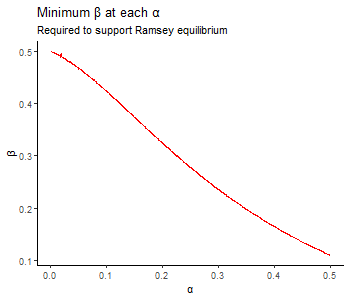
\includegraphics[scale=.75]{figure3.png}
		\end{center}
		Therefore, the Ramsey equilibrium can be supported in this economy.
		
\end{enumerate}


%%%________________________________________________________________%%%


\end{document}












